% Asset ID: A21AlgebraicMethodsPartialFractionsTikZ-001
% Asset type: TikZ diagram
% Source: CCEA A21-AF-LO001 and A21-AF-LO008; Chapter 1b Algebraic Methods evidence
% Related lesson sections: Core Theory; Worked Examples; Exam Technique Notes
% Purpose: Algebraic division layout for an improper rational function before partial fractions.
%
% Compile as a standalone LaTeX file, or paste the tikzpicture into the lesson build system.

\documentclass[tikz,border=8pt]{standalone}

\usepackage{amsmath}
\usepackage{tikz}
\usetikzlibrary{arrows.meta, positioning, fit, calc}

\begin{document}

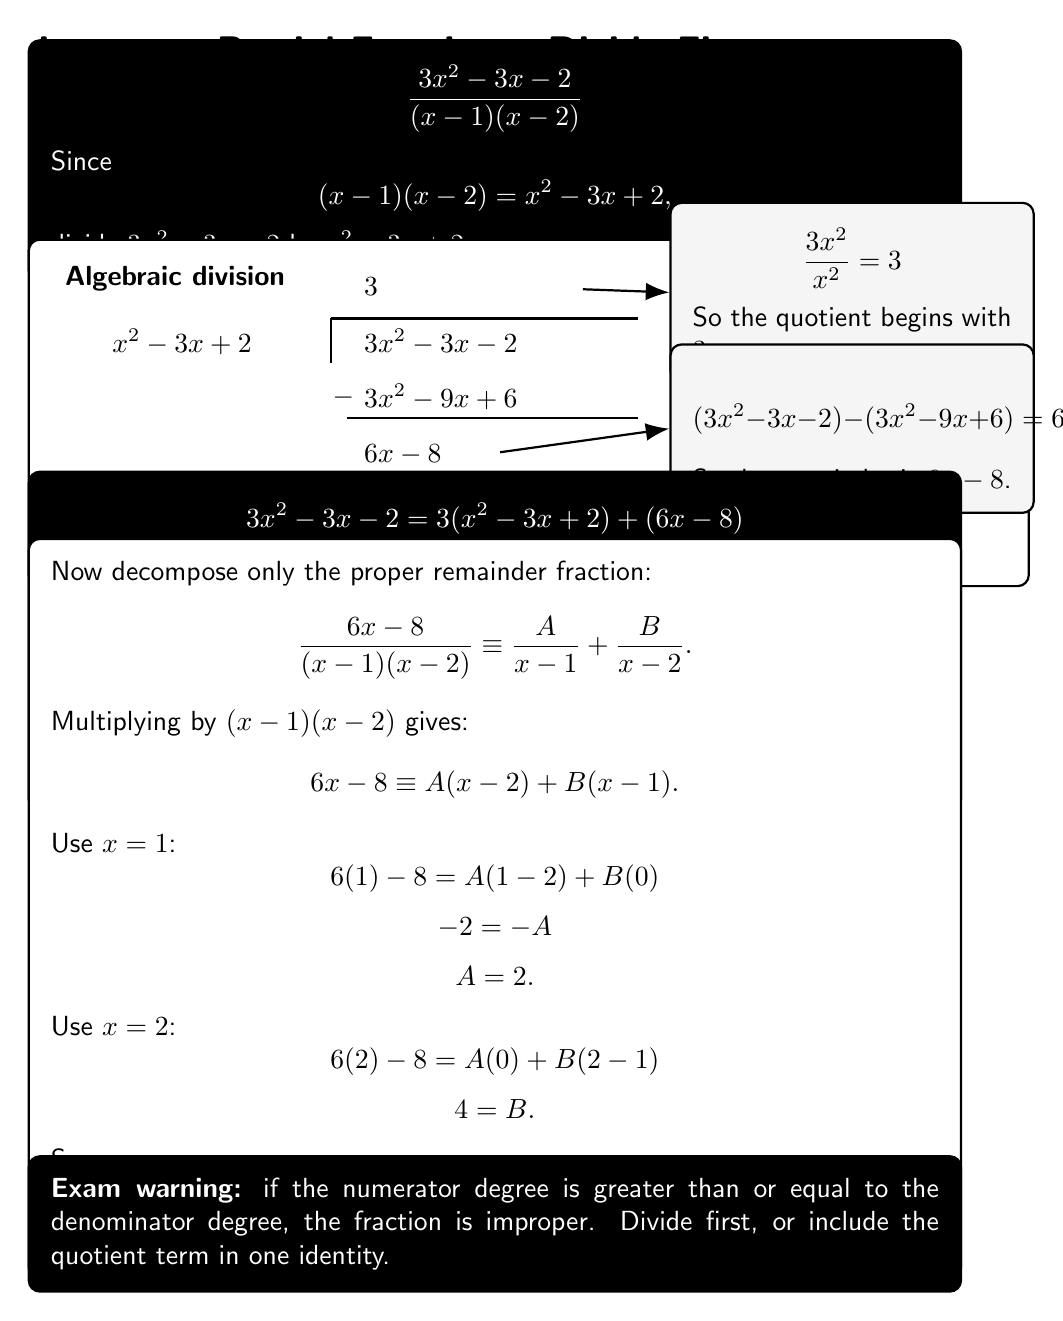
\begin{tikzpicture}[
    every node/.style={font=\sffamily},
    title/.style={font=\sffamily\bfseries\Large},
    subtitle/.style={font=\sffamily\small},
    box/.style={
        draw=black,
        rounded corners=4pt,
        line width=0.8pt,
        fill=white,
        inner sep=8pt
    },
    darkbox/.style={
        draw=black,
        rounded corners=4pt,
        line width=0.8pt,
        fill=black,
        text=white,
        inner sep=8pt
    },
    stepbox/.style={
        draw=black,
        rounded corners=4pt,
        line width=0.8pt,
        fill=gray!8,
        inner sep=8pt
    },
    arrow/.style={-{Latex[length=3mm]}, line width=0.8pt}
]

\node[title, anchor=west] at (0,0) {Improper Partial Fractions: Divide First};
\node[subtitle, anchor=west] at (0,-0.45)
{Example: rewrite an improper rational function as quotient plus proper fraction.};

\node[darkbox, anchor=west] (start) at (0,-1.35) {
\begin{minipage}{0.93\linewidth}
\[
\frac{3x^2-3x-2}{(x-1)(x-2)}
\]
Since
\[
(x-1)(x-2)=x^2-3x+2,
\]
divide \(3x^2-3x-2\) by \(x^2-3x+2\).
\end{minipage}
};

\node[box, anchor=west, minimum width=12.7cm, minimum height=4.4cm] (division) at (0,-4.55) {};

\node[anchor=west, font=\sffamily\bfseries] at (0.35,-2.85) {Algebraic division};

\node[anchor=west] at (0.95,-3.65) {\(\displaystyle x^2-3x+2\)};
\node[anchor=west] at (4.15,-3.65) {\(\displaystyle 3x^2-3x-2\)};

\draw[line width=0.9pt] (3.85,-3.35) -- (3.85,-3.92);
\draw[line width=0.9pt] (3.85,-3.35) -- (7.75,-3.35);

\node[anchor=west, font=\sffamily\bfseries] at (4.15,-2.95) {\(\displaystyle 3\)};

\node[anchor=west] at (4.15,-4.35) {\(\displaystyle 3x^2-9x+6\)};
\node[anchor=west] at (3.75,-4.35) {\(-\)};

\draw[line width=0.8pt] (4.05,-4.62) -- (7.75,-4.62);

\node[anchor=west, font=\sffamily\bfseries] at (4.15,-5.08) {\(\displaystyle 6x-8\)};

\node[stepbox, anchor=west] (qstep) at (8.15,-3.02) {
\begin{minipage}{4.05cm}
\[
\frac{3x^2}{x^2}=3
\]
So the quotient begins with \(3\).
\end{minipage}
};

\node[stepbox, anchor=west] (rstep) at (8.15,-4.75) {
\begin{minipage}{4.05cm}
\[
(3x^2-3x-2)-(3x^2-9x+6)=6x-8
\]
So the remainder is \(6x-8\).
\end{minipage}
};

\draw[arrow] (7.05,-2.98) -- (qstep.west);
\draw[arrow] (6.0,-5.05) -- (rstep.west);

\node[darkbox, anchor=west] (qrform) at (0,-7.45) {
\begin{minipage}{0.93\linewidth}
\[
3x^2-3x-2
=
3(x^2-3x+2)+(6x-8)
\]
Therefore:
\[
\frac{3x^2-3x-2}{x^2-3x+2}
=
3+\frac{6x-8}{x^2-3x+2}
\]
and since \(x^2-3x+2=(x-1)(x-2)\),
\[
\frac{3x^2-3x-2}{(x-1)(x-2)}
=
3+\frac{6x-8}{(x-1)(x-2)}.
\]
\end{minipage}
};

\node[box, anchor=west] (partial) at (0,-10.85) {
\begin{minipage}{0.93\linewidth}
Now decompose only the proper remainder fraction:
\[
\frac{6x-8}{(x-1)(x-2)}
\equiv
\frac{A}{x-1}+\frac{B}{x-2}.
\]
Multiplying by \((x-1)(x-2)\) gives:
\[
6x-8\equiv A(x-2)+B(x-1).
\]
Use \(x=1\):
\[
6(1)-8=A(1-2)+B(0)
\]
\[
-2=-A
\]
\[
A=2.
\]
Use \(x=2\):
\[
6(2)-8=A(0)+B(2-1)
\]
\[
4=B.
\]
So:
\[
\boxed{
\frac{3x^2-3x-2}{(x-1)(x-2)}
\equiv
3+\frac{2}{x-1}+\frac{4}{x-2}
}
\]
\end{minipage}
};

\node[darkbox, anchor=west] at (0,-14.85) {
\begin{minipage}{0.93\linewidth}
\textbf{Exam warning:} if the numerator degree is greater than or equal to the denominator degree, the fraction is improper.  
Divide first, or include the quotient term in one identity.
\end{minipage}
};

\end{tikzpicture}

\end{document}
